\clearpage
\subsection{Nonlinear Optimization problem}
The objective is to minimize the following cost function:
\begin{align}
(C) : \hspace{2mm}
& \mbox{minimize} \ V(x) = \mbox{ln}(x_1)- x_2 ; \ \  x \in \mathbb{R}^2 \nonumber \\
& \mbox{subject to : } \nonumber \\
& \hspace{2cm} h_1(x)= x_1 - 1  \geq 0 \nonumber \\
& \hspace{2cm} h_2(x)= x_1^2 + x_2^2 -4 = 0 \nonumber
\end{align}
This is a constrained nonlinear optimization problem of the form:
\begin{align}
    minimize \hspace{2mm} V(x) = f(x) \\
    subject\hspace{2mm} to\hspace{2mm} c(x) \geq 0 \\
    subject\hspace{2mm} to \hspace{2mm}h(x) = 0 \\
\end{align}
This can be solved using these algorithms: 
\begin{itemize}
    \item Penalty Function Algorithm
    \item Barrier Function Algorithm
    \item Augmented Lagragrian Algorithm
    \item Lagrange-Newton Algorithm
\end{itemize}
\subsubsection{Solutions to constrained nonlinear problem using our python programs and matlab benchmark \textit{fmincon} function: }
We encountered infeasible solutions full of zeros for this problem with the penalty function and augmented Lagrangian methos. The solution from the Lagrange-Newton Algorithm is very close local minimal solutions for $x$ with a tolerance set to be $tol =1e-8$ and the same initial value of all column vector of $[5,5]^{T}$ as confirmed in the contour plot in figure 11. Surprisingly, the gradient loss of the newton Lagrangian algorithm increases but settles after 2 iterations. The Matlab implementation used the quasi-Newton method approaching the minimum at 8 iterations.
The contour plot of the function $V(x)$ and the minimum solutions of $x$ derived from the newton Lagrangian algorithms showed that the lowest value of the objective function for at the intersection of the constraint ellipse and the contour plot of the objective function. 
\begin{table}[htbp]
\centering
\begin{center}
\begin{tabular}{|c|c|c|}
\hline
 &\textbf{\textit{Newton Lag}} & \textbf{Matlab}\\
\hline
Iterations & 27 & 82 \\
\hline
$x$ & 
\begin{bmatrix}
1 \\
1.732 \\
\end{bmatrix}
&\begin{bmatrix}
 1.0000  \\  1.7321 \\
\end{bmatrix}\\
\hline 
\end{tabular}
\label{table:results}
\caption{Algorithm performance}
\end{center}
\end{table}

\begin{figure}[h!]
\hfill
\begin{subfigure}[t]{0.4\textwidth}
\centering
    \includegraphics[width=\textwidth]{images/python/al-pF-ln.eps}
    \caption{}
    \label{fig:TSNE}
\end{subfigure}
\hfill
\begin{subfigure}[t]{0.4\textwidth}
\centering
    \includegraphics[width=\textwidth]{images/matlab/2c_loss.eps}
    \caption{}
    \label{fig:TSNE}
\end{subfigure}
\caption{(a): Newton Lagrangian, (d): Matlab: \textit{fmincon - interior - point}}
\end{figure}
\begin{figure}
    \centering
    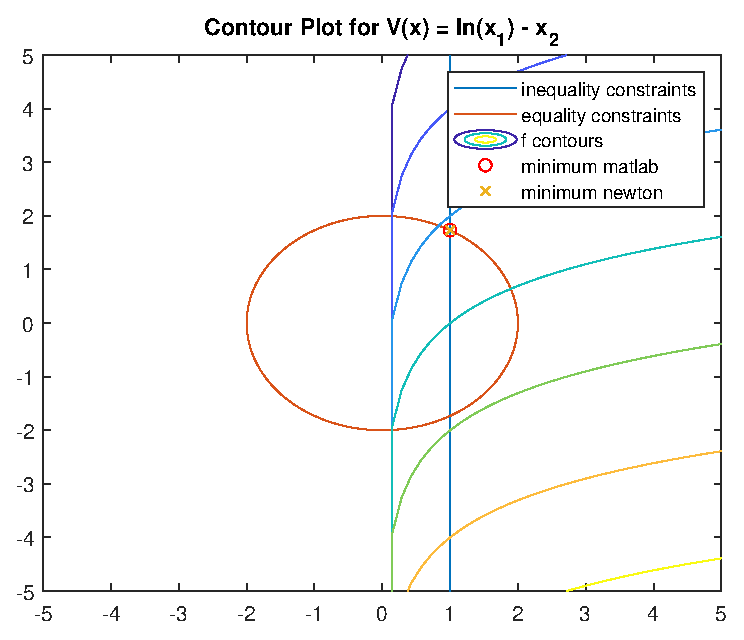
\includegraphics[width=0.4\textwidth]{images/matlab/matlab_2c.eps}
    \caption{Contour Plot for $V(x) =  V(x) = \mbox{ln}(x_1)- x_2$ and its constraints}
\end{figure}